\documentclass{article}
\usepackage[utf8]{inputenc}
\usepackage{cs-347}

\begin{document}

\thispagestyle{empty}
\titleBC

% \setcounter{section}{-1}

% \section{Notation}

\section{Process} % (fold)
\label{sec:introduction}

	\subsection{What makes a good operating system?}
	
		An \textbf{operating system} is the middleware between user programs and system hardware. It manages hardware such as the CPU, main memory, I/O devices, etc.

		When one runs a program OS, a \emph{compiler} translates high-level programs to an executable (".c" to "a.out"). This executable contains instructions that the CPU can understand and data of the program (numbered using addresses). These instructions run on a CPU -- the hardware implements an \emph{instruction set architecture} (ISA). The CPU also has a few registers, a pointer to the current instruction (known as the \textbf{program counter}) and a few others such as operands of instructions, and memory addresses.

		So, what happens When we run an executable, the CPU
		\begin{itemize}
			\item \emph{fetches} the instruction pointed at by the PC from memory,
			\item loads the data required by the instructions,
			\item \emph{decodes} and \emph{executes} the instruction, and
			\item stores the result back to memory.
		\end{itemize}
		The above is known as the \emph{Von Neumann} model of computing.\\
		Further, recently used instructions and data are stored in an instruction cache (I - cache) and data cache ( D - cache) for fast access.\\

		Where does the OS fit into this picture? It
		\begin{itemize}
			\item manages program memory by loading the program executable (code, data) from disk to the memory.
			\item manages the CPU by initializing the PC and other registers to ready for execution.
			\item manages external devices such as reading/writing files from/to the disk.
		\end{itemize}
		Due to this, an OS is also sometimes known as a \emph{resource manager}.\\

		The OS provides a \emph{process abstraction} -- it creates and manages processes (a running program) so that you can run your program on the computer system. Each process is under the illusion of having access to the complete CPU since the OS \emph{virtualizes} the CPU. It also timeshares the CPU between and coordinates multiple processes. Also enables coordination between processes\\

		The OS manages the memory of the process, including code (compiled instructions written by the user), data (variables created by the user), stack (storage of arguments/return addresses from function calls), heap (\texttt{malloc}s for example), etc.\\
		Individual processes think they have dedicated memory space for themselves, with numbers, code, and data starting from $0$ (\textbf{virtual addresses}). The OS abstracts out details of the actual placement in memory, translating between virtual addresses (which the process sees) and physical addresses (actual addresses in the hardware).\\

		The OS also has a piece of OS kernel code (\textbf{device drivers}) to communicate with hardware devices such as disk and network cards. They issue instructions to devices (fetching data from a file, for example) and respond to interrupt events from devices (when the user has pressed a key on a keyboard, for example). Everything is there in OS itself so that anyone who writes a program doesn't worry about how to write the language of this particular device. Persistent data is organized as a \emph{file system} on disk.\\

		What do we want when designing an OS?
		\begin{itemize}
			\item Convenience via abstraction of hardware resources for user programs. The primary goal of OS.
			\item Efficiency of usage of CPU, memory, etc.
			\item Isolation of multiple processes (so one program cannot interfere with another).
		\end{itemize}
		That is, we want virtualization to be effective and secure.

		Operating systems started out as just a library to provide common functionality across programs. Later, we evolved from procedure calls to system calls -- these are called when we want to run OS code and are executed at a higher privilege level. These interfaces between the OS and the user are called \emph{APIs}. It also evolved from running a single program to multiple processes concurrently.

	\subsection{Process abstractions}

		When we run an executable, the OS creates a process, a running program, virtualizing the CPU and time-sharing it across processes. The OS has a \emph{CPU scheduler} that picks one of the several active processes to execute, which has two parts: the \textbf{policy} that decides which process to run and the \textbf{mechanism} which knows how to ''context switch'' between processes and ensures that the process chosen to run is running.\\

		Any process created has a unique identifier, known as the \emph{process ID} (PID).\\
		It also has a certain memory footprint or \emph{memory image}, consisting of the code (compiled instruction) and data, which are static, and the stack and heap, which are dynamic. The stack is used for function calls and function arguments, while the heap is used for dynamic memory allocation (\texttt{malloc}s in C for instance). These resides in RAM.\\
		It has a \emph{CPU context}, which consists of the registers used in the process -- the program counter (which points to the current position in the code), current operands (which looks at the data), and stack pointer (which points to the current position in the stack).\\
		Finally, have bunch of open file. File descriptors that are pointers to open files/devices. \texttt{stdout} and \texttt{stdin} are examples of this.\\

		How does OS creates a process?
		\begin{itemize}
			\item it allocates memory and creates a memory image. This loads code and data from a disk executable, and creates the runtime stack and heap.
			\item it opens some basic files for the program such as \texttt{stdin}, \texttt{stdout}, and \texttt{stderr} for example.
			\item it initializes various registers such as the PC which should point to the first instruction.
		\end{itemize}

		The primary states that any process is in are:
		\begin{itemize}
			\item \emph{running} -- currently executing on the CPU.
			\item \emph{ready} -- waiting to be scheduled.
			\item \emph{blocked} -- suspended, not ready to run. This may be because they are waiting for some event (such as a read from a disk). They can eventually be unblocked when the event is done (when the disk issues an interrupt, for example).
			\item \emph{new} -- being created and is yet to run.
			\item \emph{dead} -- terminated processes.		
		\end{itemize}
		
        Process State Transitions
		\begin{center}
		    \begin{tikzpicture}[node distance=4cm]
		    \node[state] (q1) {Running};
		    \node[state, below right of=q1] (q2) {Blocked};
		    \node[state, above right of=q2] (q3) {Ready};

		    \draw (q1) edge[bend left, above] node{Descheduled} (q3)
		          (q3) edge[bend left, below] node{Scheduled} (q1)
		          (q1) edge[bend right, below left] node{I/O: initiate} (q2)
		          (q2) edge[bend right, below right] node{I/O: done} (q3);
		    \end{tikzpicture}
		\end{center}
        OS data Structures
        
		The OS maintains a data structure (a list)	 of all active processes. Information about each process is stored in a \textbf{process control block} (PCB) which has the
		\begin{itemize}
			\item process identifier,
			\item process state,
			\item pointers to other related processes (parent for example),
			\item CPU context of the process (which is saved when the process is suspended),
			\item pointers to memory locations, and
			\item pointers to open files.
		\end{itemize}	

\subsection{Process API}

What does an \textbf{API} mean? \textbf{API} stands for Application Programming Interface and it is simply a function available to users to write user programs. What API does the OS provide to user
programs? API provided by OS is a set of "system calls". What does "system calls" mean? A system calls a function call into OS code that runs at a \emph{higher privilege} level of the CPU. Sensitive operations (e.g., access to hardware) are allowed only at a higher privilege level. Some “blocking” system calls cause the process to be blocked and descheduled (e.g., read from disk).\\

So, should we rewrite programs for each OS?

\textbf{POSIX API}: a standard set of system calls that an OS must implement – Programs written to the POSIX API can run on any POSIX-compliant OS.
Program language libraries hide the details of invoking system calls – The printf function in the C library calls the writing system call to write to the screen. $C \rightarrow libc \rightarrow systemcall$\\

\texttt{How printf works in C internally on linux?}

The printf function (the name comes from “print formatted”) prints a string on the screen using a "format string" that includes the instructions to mix several strings and produce the final string to be printed on the screen.
\begin{itemize}
    \item A kernel runs in ring 0, meaning it has full access to memory and opcodes. A program runs usually in ring 3. It has limited access to memory, and cannot use all the opcodes.

    \item Interrupts, with the printf() function. Our program calls printf() $\mathbf{\rightarrow}$ printf() processes string, and args, and then needs to execute a kernel function, as writing to a file can't be done in ring 3. $\rightarrow$ printf() generates a software interrupt, placing in a register the number of a kernel function (in that case, the write() function). $\rightarrow$ The program execution is interrupted, and the instruction pointer moves to the kernel code. So we are now in ring 0, in a kernel function. $\rightarrow$ The kernel process the request, writing to the file (stdout is a file descriptor). $\rightarrow$ When done, the kernel returns to the program's code, using the iret instruction.
\end{itemize}

\subsubsection{Process related system calls (in Unix)}
\begin{itemize}
    \item \texttt{fork() system call}: used to create a new child process.
    \begin{center}
		    \begin{tikzpicture}[node distance=4cm]
		    \node[state] (q1) {init};
		    \node[state, below left of=q1] (q2) {login};
		    \node[state, below of=q1] (q3) {kthread};
              \node[state, below right of=q1] (q4) {sshd};

		    \draw (q1) edge[below] (q2)
		          (q1) edge[below] (q3)
		          (q1) edge[below] (q4);
		    \end{tikzpicture}
    \end{center}
    \texttt{init} is the ancestor of all processes.

    The child process that is created is an (almost) exact copy of the calling process. both are about to return from the fork() system call[fork() return pid of child process in calling process and 0 in child process). The child process doesn’t start running at main(), like we might expect. 

    Parent and child execute and modify the memory data independently. The child isn’t an exact copy. Specifically, although it now has its own copy of the address space (i.e., its own private memory), its own registers, its own PC, and so forth, the value it returns to the caller of fork() is different.
    \item \texttt{exit()} terminates a process. exit is called automatically when the end of the main is reached. Also, OS terminates a misbehaving process

    Processes may also be terminated by the system for a variety of reasons, including:
    \begin{itemize}
        \item The inability of the system to deliver necessary system resources.
        \item In response to a KILL command, or other unhandled process interrupts.
        \item A parent may kill its children if the task assigned to them is no longer needed.
        \item If the parent exits, the system may or may not allow the child to continue without a parent. ( On UNIX systems, orphaned processes are generally inherited by init, which then proceeds to kill them. The UNIX \texttt{nohup} command allows a child to continue executing after its parent has exited. )
    \end{itemize}

    \item \texttt{wait() or its sibling waitpid()}: causes a parent to block(non-blocking ways also exist - "WNOHANG" checks child processes without causing the caller to be suspended) until child terminates. Terminated process exists as a zombie When a parent calls wait(), zombie child is cleaned up or "reaped".
    \texttt{What if parent terminates before child?}
    
    init process adopts orphans and reaps them. Note that modern UNIX shells do not produce as many orphans and zombies as older systems used to.

    \item \texttt{exec()} makes a process execute a given executable. After fork, parent and child
    runs same code, not very useful. It will make more sense to run another executable in the child process - thats what exec do. A process can run exec() to load another executable to its
    memory image. 

    Note that all statements below the exec statement in the calling process will not get executed in case exec successful. Ofcourse, it gets executed if exec failed for any reason. it does not
    create a new process; rather, it transforms the currently running program
\end{itemize}

\subsubsection{Process Control And Users}
\texttt{kill()} system call is used to send signals to a process, including directives to pause, die, and other useful imperatives. For convenience, in most UNIX shells, certain keystroke combinations are configured to deliver a specific signal to the currently running process; for example, \textbf{control-c} sends a \texttt{SIGINT} (interrupt) to the process (normally terminating it) and \textbf{control-z} sends a \texttt{SIGTSTP} (stop) signal thus pausing the process in mid-execution (you can resume it later with a command, e.g., the \texttt{fg} built-in command found in many shells).\\

\textbf{control-\textbackslash}: Pressing this key causes the system to send an \texttt{ABRT} signal (SIGABRT) to the running process. By default, this signal causes the process to terminate immediately. Note that this redundancy (i.e. Ctrl-\textbackslash doing the same as Ctrl-C) gives us some flexibility.
We can override the default signal handler to IGN (ignore) or write our own custom handler. This is useful if we would like our program to react differently to certain kinds of signals.\\

Signal: \texttt{SIGCHLD} $\rightarrow$ Description: When a child changes state, the kernel sends a \texttt{SIGCHLD} signal to its parent $\rightarrow$ Default Action: Ignore.
Note1: Signals aren't Queued, a signal handler is called if one or more signals are sent.
Note2: If you are generating the SIGINT with \textbf{control-c} on a Unix system, then the signal is being sent to the entire process group.

%%%%%% Lecture 4 %%%%%
\subsection{Mechanism of process execution: Limited Direct Execution}
\subsubsection{Low-level mechanisms}
Some important questions we need to know...
\begin{itemize}
    \item How does the OS runs the process?
    \item How does it handle a system call?
    \item How does it context switch from one process to the other?
    \item How can we virtualize the CPU?

    The OS needs to somehow share the physical CPU among many jobs running seemingly at the same time. The basic idea is simple: run one process for a little while, then run another one, and so forth. By \textbf{time sharing} the CPU in this manner, virtualization is achieved.

    There are a few challenges, however, in building such virtualization machinery. The first is performance and the second is control: Control is particularly important to the OS, as it is in charge of resources; without control, a process could simply run forever and take over the machine, or access information that it should not be allowed to access.

    
\end{itemize}
\textcolor{red}{more details later...}

\subsubsection{Process Execution}
Two modes of process execution: user mode and kernel mode

Normally, a process executes in user mode. When a process executes a system call, the mode of execution changes from user mode to kernel mode. The bookkeeping operations related to the user process (interrupt handling, process scheduling, memory management) are performed in kernel mode.\\

The process is an instance of a program in execution. OS allocates memory and
creates memory image. Process memory is divided into four sections: Code \textit{\&} data (from exe) and Stack \textit{\&} heap. Points CPU program counter to current instruction and Other registers may store operands, return values etc. After setup, OS is out of the way and the process executes directly on CPU.

\subsection{Scheduling Policies(disciplines)}
What is a scheduling policy? On the context switch, which process to run next, from the set of ready processes?

OS scheduler schedules the CPU requests(bursts) of processes. CPU burst = the CPU time used by a process in a continuous stretch. If a process comes back after I/O wait, it counts as a fresh CPU burst

\subsubsection{Scheduling Metrics}
\begin{itemize}
    \item \texttt{Turnaround Time}: performance metric
        $$T_{turnaround} = T_{completion} - T_{arrival}$$

    \item \texttt{Response Time}:
        $$T_{response} = T_{firstrun} - T_{arrival}$$

    \item \texttt{fairness} as measured (for example) by Jain’s Fairness Index. all processes must be treated equally

    \item \texttt{utilization} = fraction of time CPU is used
\end{itemize}
\texttt{What are we trying to optimize?}

We want to maximize utilization, minimize average turnaround time, minimize average response time, as much fairness as possible and minimize overhead: run process long enough to amortize the cost of context switch (\texttt{~}1 microsecond).

\subsubsection{First In, First Out(FIFO)}
Sometimes also called First Come, First Served. It is simple and thus easy to implement.
\begin{figure}[H]
        \centering
        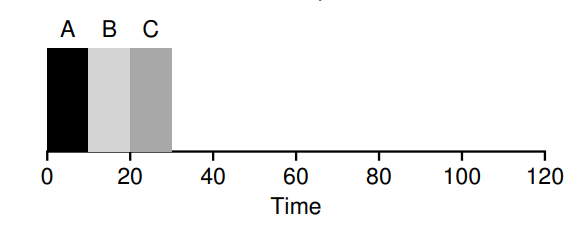
\includegraphics[width=0.6\linewidth]{image/fifo1.png}
        \caption{FIFO simple example}
\end{figure}
Imagine three jobs arrive in the system, A, B, and C, at roughly the same time ($T_{arrival} = 0$). Because FIFO has to put some job first, let's assume that while they all arrived simultaneously, A arrived just a hair before B which arrived just a hair before C. Assume also that each job runs for 10 seconds.

$$\text{Average Turnaround Time} = \frac{10 + 20 + 30}{3} = 20$$
\begin{figure}[H]
        \centering
        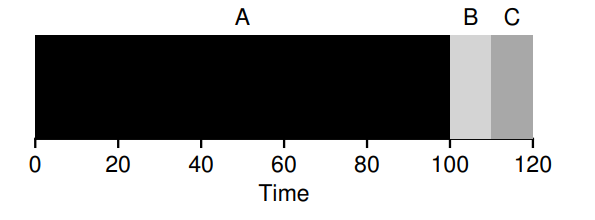
\includegraphics[width=0.6\linewidth]{image/fifo2.png}
        \caption{Why FIFO is not that good?}
\end{figure}

In the Figure2, Turnaround times tend to be high. This problem is generally referred to as \textbf{convoy effect} - when a relatively short resource consumer process is stuck behind a heavyweight resource consumer.

\subsubsection{Shortest Job First(SJF)}
It runs the shortest job first, then the next shortest, and so on. Probably optimal when all jobs arrive together.

\begin{figure}[H]
        \centering
        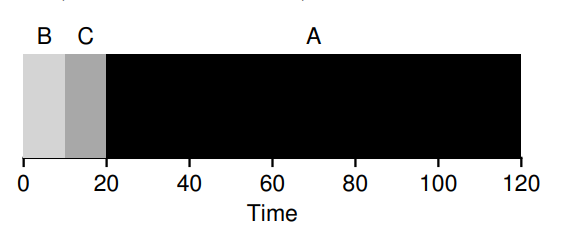
\includegraphics[width=0.6\linewidth]{image/sjf1.png}
        \caption{SJF simple example}
\end{figure}
We arrive at a good approach to scheduling with SJF, but our assumptions(all jobs arrive together) are fairly unrealistic.

$$\text{Average Turnaround Time} = \frac{10 + 20 + 30}{3} = 20$$
\begin{figure}[H]
        \centering
        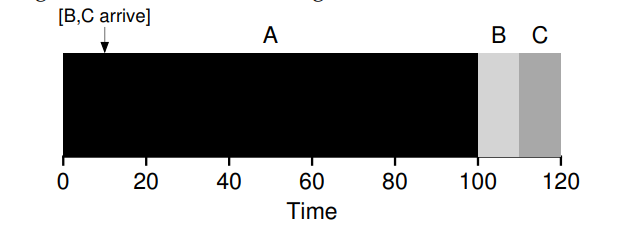
\includegraphics[width=0.6\linewidth]{image/sjf2.png}
        \caption{SJF With Late Arrivals From B and C}
\end{figure}
SJF is \textbf{non-preemptive}(non-preemptive systems would run each job to completion before considering whether to run a new job), so short jobs can still get stuck behind long ones(i.e Figure 4) and suffer the same convoy problem.

\subsubsection{Shortest Time-to-Completion First(STCF)}
Also called Shortest Remaining Time First (SRTF) or Preemptive Shortest Job First (PSJF)$\rightarrow$ Preemptive scheduler $\rightarrow$ Preempts running task if time left is more than that of a new arrival.

Any time a new job enters the system, the STCF scheduler determines which of the remaining jobs (including the new job) has the least time left, and schedules that one. 
\begin{figure}[H]
        \centering
        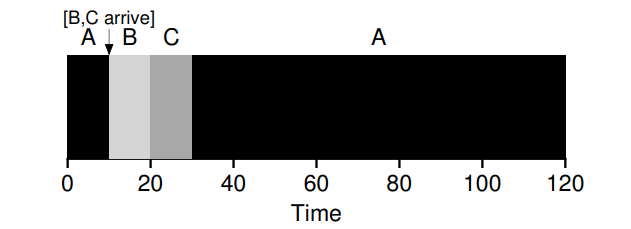
\includegraphics[width=0.6\linewidth]{image/stcf.png}
        \caption{STCF simple example}
\end{figure}
Thus, in Figure 5, STCF would preempt A and run B and C to completion; only when they are finished would A's remaining time be scheduled.

\subsubsection{Round Robin - Preemptive}
\begin{figure}[H]
        \centering
        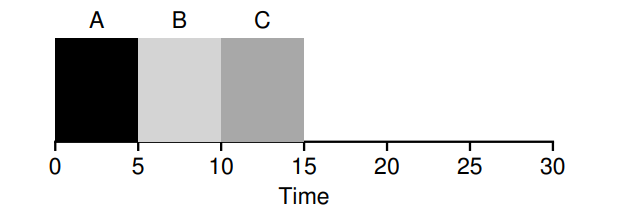
\includegraphics[width=0.4\linewidth]{image/sjf3.png}
        \caption{SJF Again! (Bad for Response Time)}
\end{figure}
Instead of running jobs to completion(SJF), RR runs a job for a time slice (sometimes called a scheduling quantum) and then switches to the next job in the run queue. It repeatedly does so until the jobs are finished. For this reason, RR is sometimes called \textbf{time-slicing}. Note that
the length of a time slice must be a multiple of the timer-interrupt period. Slice big enough to
amortize the cost of the context switch.
\begin{figure}[H]
        \centering
        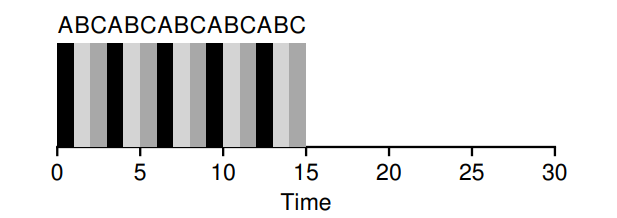
\includegraphics[width=0.6\linewidth]{image/rr.png}
        \caption{RR - Good for response time}
\end{figure}

\begin{itemize}
    \item Good for response time and fairness.
    \item Bad for turn around time
\end{itemize}

\textcolor{red}{some more scheduling policies}
\subsubsection{Priority Based Scheduling}
In this scheme, each process is associated with a "priority" value. The scheduler ensures the use of process priority in picking the next process to schedule. The idea is as follows: assign each running process a priority, which is a non-negative integer number (the higher the number, the higher will be its priority).\\

Each time the scheduler runs, the scheduler should run processes that have a high priority. If there are two or more processes that have the same high priority, the scheduler should loop over the processes with high priority and choose the first which is available. A low-priority process does NOT run as long as there are higher-priority processes waiting to run.

\subsubsection{Multilevel Queue Scheduling (MLQ)}
According to the priority of the process, processes are placed in different queues. Generally, high-priority processes are placed in the top-level queue. Only after the completion of processes from the top-level queue, are lower-level queued processes scheduled.

\subsubsection{Multilevel Feedback Queue (MLFQ) Scheduling}
\textcolor{blue}{ In fact, in a general-purpose OS (like the ones we care about), the OS usually knows very little about the length of each job. Thus, how can we build an approach that behaves like SJF/STCF without such a \textit{priori} knowledge?}

Real schedulers are more complex.

MLFQ allows the process to move in between queues. Many queues, in order of priority – Process from highest priority queue scheduled first. Within the same priority, any algorithm like RR – Priority of process decays with its age. If a process uses too much CPU time, it is moved to a lower-priority queue.

\subsubsection{Incorporating I/O}
Of course, all programs perform I/O. A scheduler clearly has the decision to make when a job initiates an I/O request because the currently-running job won't be using the CPU during the I/O; it is blocked waiting for I/O completion. If the I/O is sent to a hard disk drive, the process might be blocked for a few milliseconds or longer, depending on the current I/O load of the drive. Thus, the scheduler should probably schedule another job on the CPU at that time.\\

\begin{figure}[H]
        \centering
        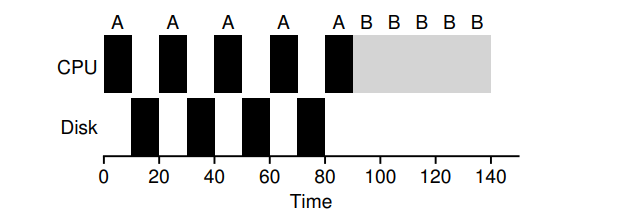
\includegraphics[width=0.6\linewidth]{image/io1.png}
        \caption{Poor Use of resources}
\end{figure}

The scheduler also has to make a decision when the I/O completes. When that occurs, an interrupt is raised, and the OS runs and moves the process that issued the I/O from blocked back to the ready state. Of course, it could even decide to run the job at that point. How should the
OS treat each job?

\begin{figure}[H]
        \centering
        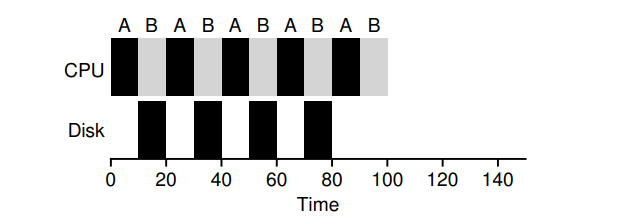
\includegraphics[width=0.6\linewidth]{image/io2.png}
        \caption{Overlap Allows Better Use Of Resources}
\end{figure}
Thus we see how a scheduler might incorporate I/O. By treating each CPU burst as a job, the scheduler makes sure processes that are "interactive" get run frequently. While those interactive jobs are performing I/O, other CPU-intensive jobs run, thus better utilizing the processor.

\subsection{Inter Process Communication (IPC)}
\begin{itemize}
    \item Processes do not share any memory with each other
    \item Some processes might want to work together for a task, so need to communicate information
    \item IPC mechanisms to share information between processes
\end{itemize}
There are two key ways we will learn to do this: pipes and signals
Pipes let two processes send and receive arbitrary data


\subsubsection{Signals}
Signals let two processes send and receive certain "signals" that indicate something special has happened.

Signals Sources
\begin{itemize}
    \item Hardware - division by zero
    \item Kernel – notifying an I/O device for which a process has been waiting is available
    \item Other Processes – a child notifies its parent that it has terminated
    \item User – key press (i.e., Ctrl-C)
    \item sources
        \begin{center}
		    \begin{tikzpicture}[node distance=6cm]
		    \node[state] (q1) {Process};
		    \node[state, above left of=q1] (q2) {Shell Cmnd};
		    \node[state, above of=q1] (q3) {Terminal Driver};
              \node[state, above right of=q1] (q4) {Memory Manager};
              		    \node[state, below left of=q1] (q5) {Kernel};
		    \node[state, below of=q1] (q6) {user Process};
              \node[state, below right of=q1] (q7) {Window Manager};

		    \draw (q2) edge[bend right, below] node{SIGKILL} (q1)
		          (q3) edge[below] node{SIGINT, SIGQUIT, SIGHUP} (q1)
                    (q4) edge[bend left, below] node{SIGSEGV}(q1)
                    (q5) edge[bend left, below] node{SIGPIPE, SIGALRM} (q1)
		          (q6) edge[below] node{SIGUSR1}(q1)
            (q7) edge[bend right, below] node{SIGWINCH}(q1);

          
		    \end{tikzpicture}
    \end{center}
\end{itemize}

Signals are defined in \texttt{/usr/include/signal.h}

A programmer may choose that
\begin{itemize}
    \item particular signal triggers a user-defined signal handler
    \item triggers the default kernel-supplied handler
    \item signal is ignored
\end{itemize}

\textbf{Process Groups}

Q. What happens when you Control-C a program that created several children?

A. Typically the program and its children terminate. Why the children? In addition to having unique ID(PID), the process also belongs to a process group.
\begin{itemize}
    \item Several processes can be members of the same process group.
    \item When a process forks, the child inherits its process group from its parent.
    \item A process may change its process group to a new value by using \texttt{setpgid ()}.
    \item When a process execs, its process group remains the same.
    \item When a metacharacter such as a Control-C is detected, the terminal sends the appropriate signal to all of the processes in the process group of its control process. Every process can have an associated control terminal. This is typically the terminal where the process started. When a process forks, the child inherits its control terminal from its parent. When a process execs, its control terminal stays the same. Every terminal can be associated with a single control process.
\end{itemize}

\subsubsection{Sockets}
\begin{itemize}
    \item Sockets can be used for two processes on the same machine or different machines to communicate
    \begin{itemize}
        \item TCP/UDP sockets across machines
        \item Unix sockets in local machine
    \end{itemize}
    \item Communicating with sockets 
    \begin{itemize}
        \item Processes open sockets and connect them to each other
        \item Messages written into one socket can be read from another
        \item OS transfers data across socket buffers
    \end{itemize}
\end{itemize}

\subsubsection{Shared Memory}
\begin{itemize}
    \item  Shared Memory allows two or more processes to share a given region of memory – this is the FASTEST form of IPC because the data does not need to be copied between communicating processes
    \item The only trick in using shared memory is synchronizing access to a given region among multiple processes – if the server/producer process is placing data into a shared memory region, the client/consumer process shouldn't try to access it until the server is done
    
    \item Need to take care that one is not overwriting other's data: how? Often, semaphores are used to synchronize shared memory access
    
    \item Processes can both access the same region of memory via shmget()system call: 
    
    \texttt{int shmget( key\_t key, int size, int shmflg )}
    \item By providing the same key, two processes can get the same segment of memory
\end{itemize}

\subsubsection{Pipes}
Conceptually, a pipe is a connection between two processes, such that the standard output from one process becomes the standard input of the other process. It is possible to have a series of processes arranged in a pipeline, with a pipe between each pair of processes in the series.\\

\textcolor{blue}{unnamed pipe}

Also called an anonymous pipe (or simply a pipe), this type of pipe is always one way. It is typically used to communicate between a parent process and a child process.\\

\textcolor{blue}{named pipe}

This type of pipe can handle one-way or two-way communication between two unrelated processes. That is, one process is not started by the other. In fact, it is possible to have two applications communicate over a pipe on a network. 

\begin{itemize}
    \item Pipe system call returns two file descriptors
    \begin{itemize}
        \item Read handle and write handle
        \item A pipe is a half-duplex communication
        \item Data written in one file descriptor can be read through another
    \end{itemize}
    \item Regular pipes: both fd are in the same process (how it is useful?) $\rightarrow$ Parent and child share fd after fork $\rightarrow$ Parent uses one end and child uses other ends
\end{itemize}

\subsubsection{Message Queues}
Mailbox abstraction $\rightarrow$ Process can open a mailbox at a specified location $\rightarrow$ Processes can send/receive messages from mailbox $\rightarrow$ OS buffers messages between send and
receive

\subsubsection{Blocking vs. non-blocking communication}
\begin{itemize}
    \item Some IPC actions can block
    \begin{itemize}
        \item Reading from socket/pipe that has no data, or reading from the empty message queue
        \item Writing to a full socket/pipe/message queue
    \end{itemize}
    \item The system calls to read/write have versions that block or can return with an error code in case of failure. A socket read can return an error indicating no data to be read, instead of blocking
\end{itemize}
% section introduction (end)

% section xv6 (start)

\section{Memory} % (fold)
\label{sec:memory}

\section{Concurrency} % (fold)
\label{sec:con}

\end{document}